\documentclass[pdf,15pt]{beamer}
\mode<presentation>{\usetheme{Warsaw}}
\usepackage{fontspec}   %加這個就可以設定字體
\usepackage{xeCJK}       %讓中英文字體分開設置

%
\usepackage{graphicx} % Allows including images
\usepackage{booktabs} % Allows the use of \toprule, \midrule and \bottomrule in tables
\setCJKmainfont{LiHei Pro} %設定中文為系統上的字型,而英文不去更動,使用原TeX字型
\XeTeXlinebreaklocale "zh"             %這兩行一定要加,中文才能自動換行
\XeTeXlinebreakskip = 0pt plus 1pt     %這兩行一定要加,中文才能自動換行

%% preamble
\title{Git \& Github}
\author{曹又霖}

\defbeamertemplate{footline}{centered page number}
{%
  \hspace*{\fill}%
  \usebeamercolor[fg]{page number in head/foot}%
  \usebeamerfont{page number in head/foot}%
  \insertpagenumber%
  \hspace*{\fill}\vskip2pt%
}

\setbeamertemplate{footline}[centered page number]
\setbeamertemplate{caption}[numbered]

\begin{document}

  %% title frame
  \begin{frame}
    \titlepage
  \end{frame}
  
  \begin{frame}
    \frametitle{大綱} % Table of contents slide, comment this block out to remove it
    \tableofcontents % Throughout your presentation, if you choose to use \section{} and \subsection{} commands, these will automatically be printed on this slide as an overview of your presentation
  \end{frame}
  
  \begin{section}{版本控制}
    \begin{subsection}{簡介}
      %% normal frame
      \begin{frame}{為什麼要版本控制}
        \begin{itemize}
          \item 改錯程式或誤刪檔案
          \item 還原之前寫的版本
          \item 團隊合作開發
          \item 軟體發行時,要分成穩定版和開發版
        \end{itemize}
      \end{frame}
    \end{subsection}
    
    \begin{subsection}{版本控制總類}
      \begin{frame}{本地端版本控制}
        \begin{figure}[h!]
          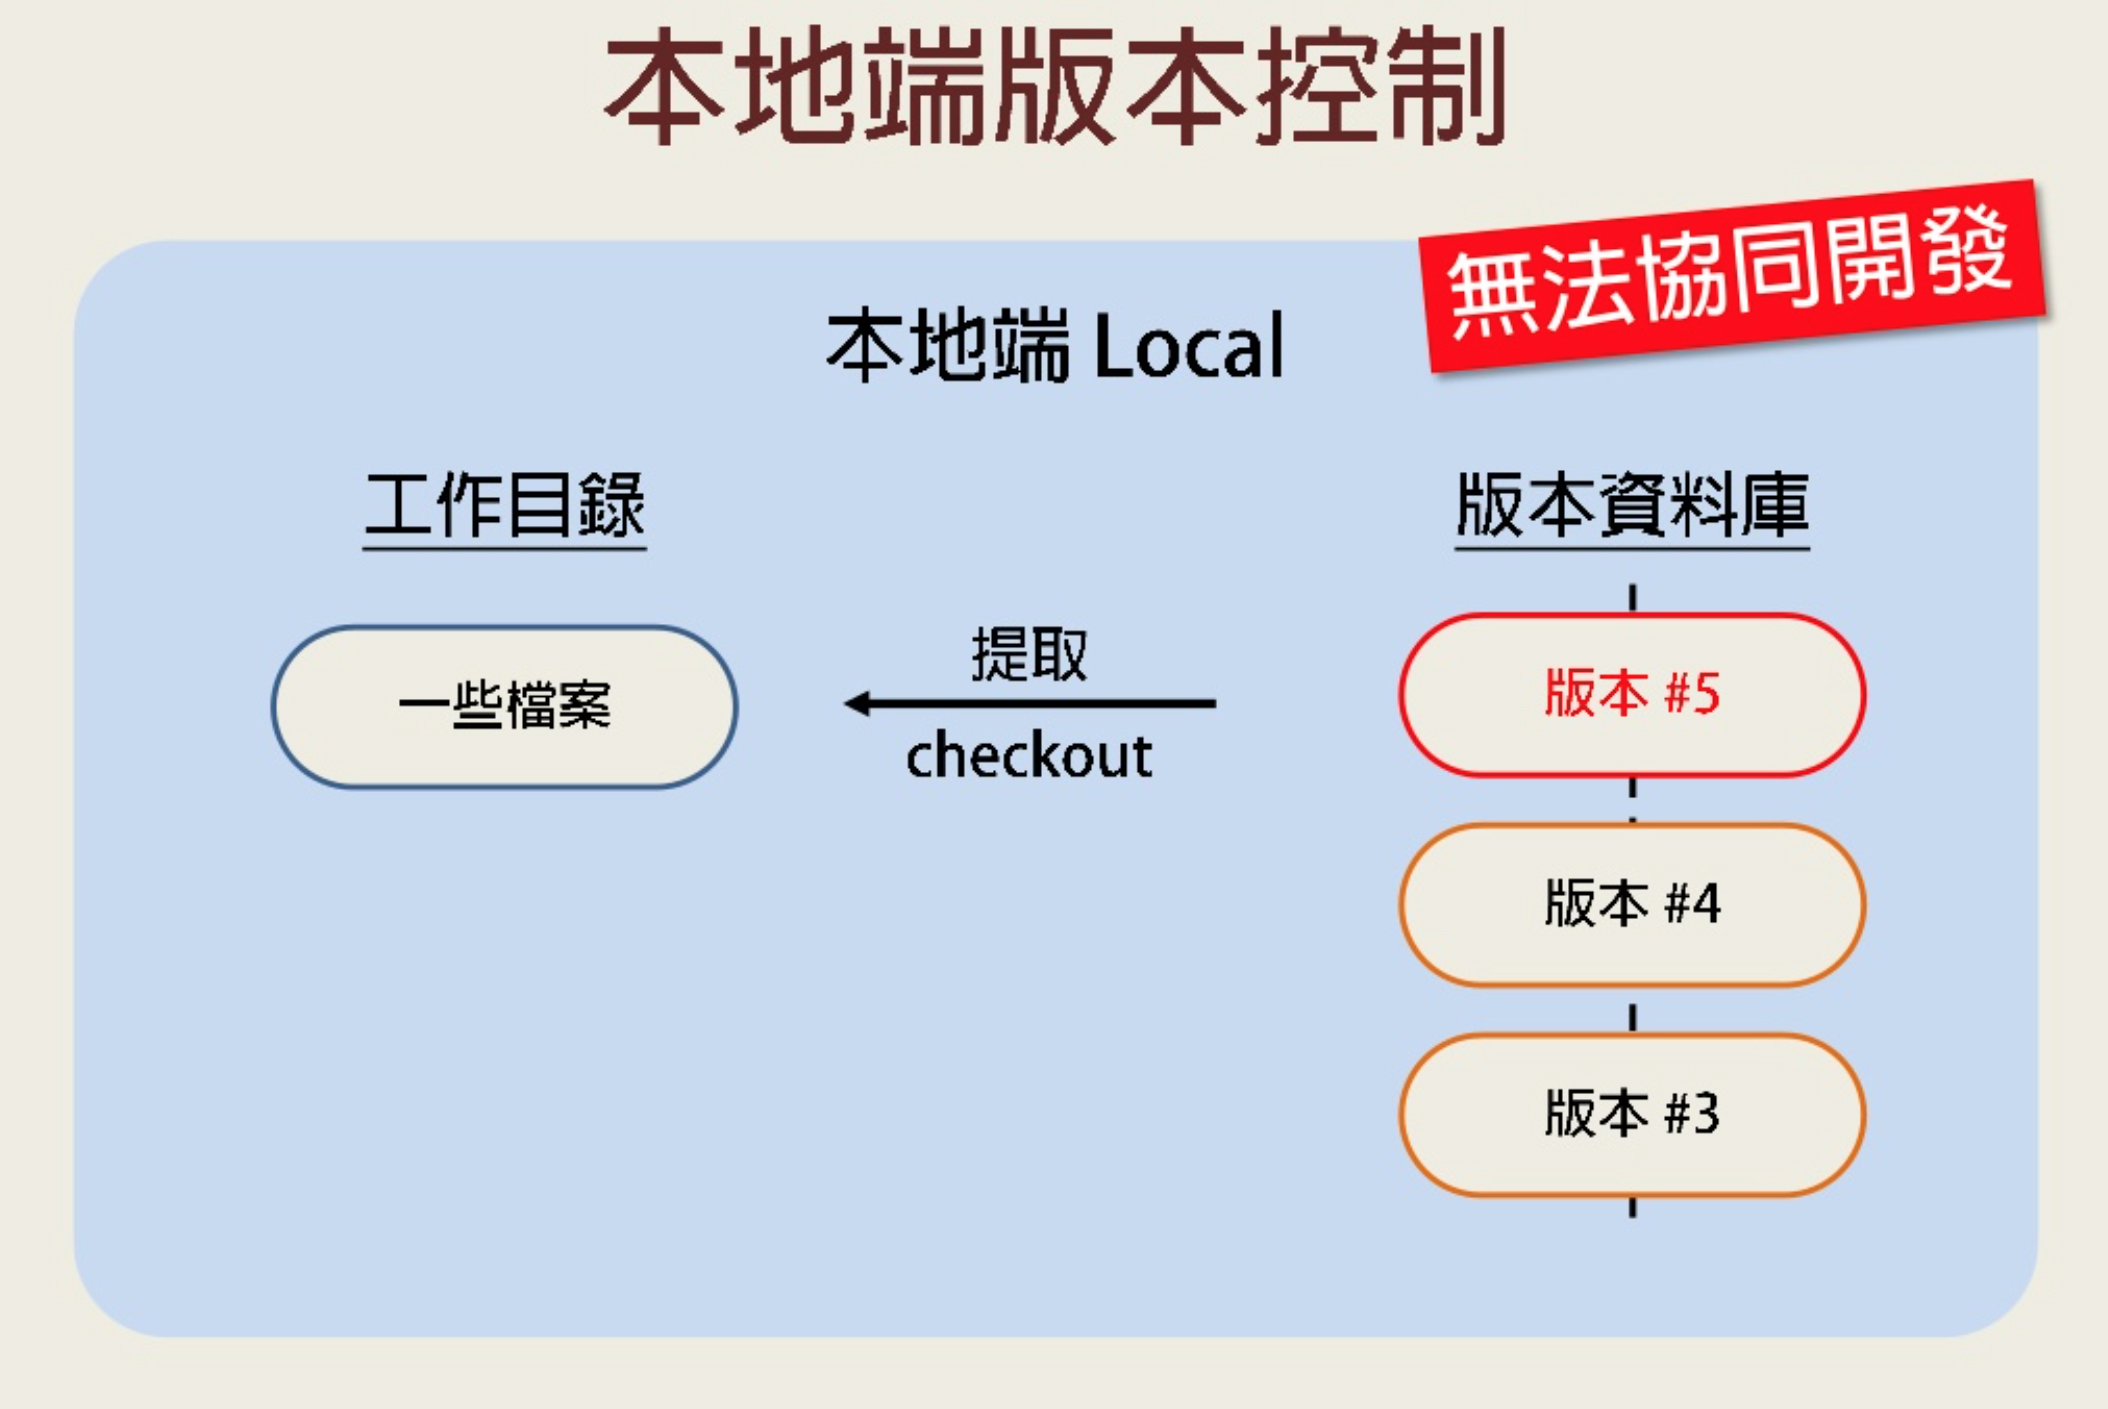
\includegraphics[width=0.8\textwidth]{images/001.jpg} 
          \caption{本地端版本控制}
        \end{figure}
      \end{frame}
      
      \begin{frame}{中心式版本控制}
        \begin{figure}[h!]
          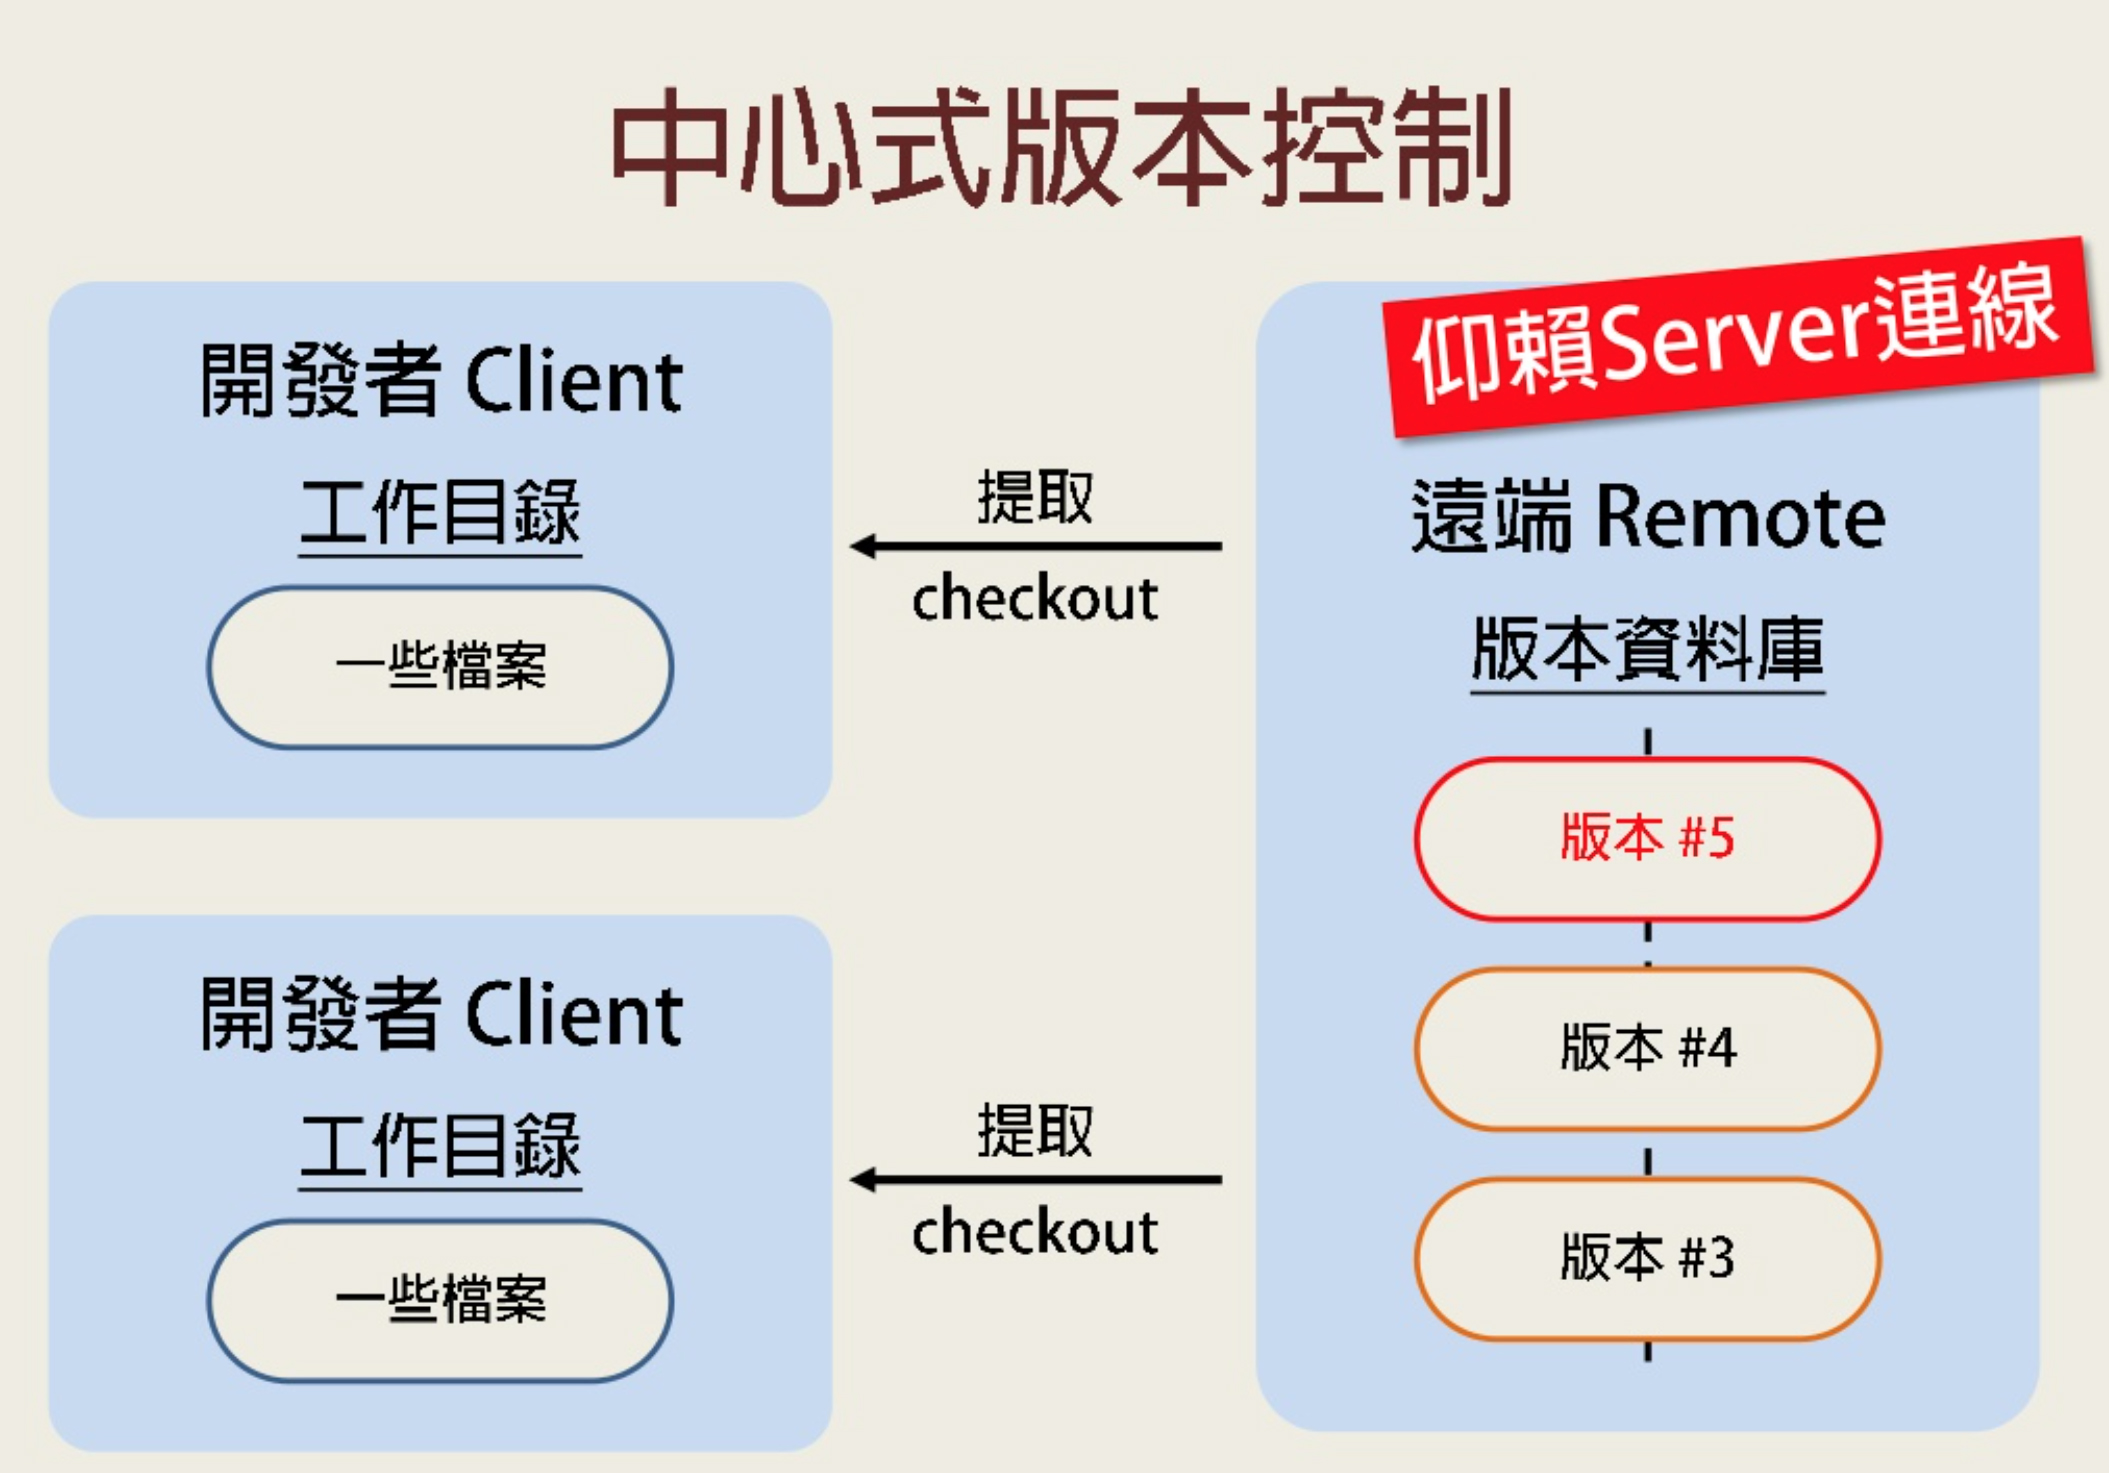
\includegraphics[width=0.8\textwidth]{images/002.jpg} 
          \caption{中心式版本控制}
        \end{figure}
      \end{frame}
      
      \begin{frame}{分散式版本控制}
        \begin{figure}[h!]
          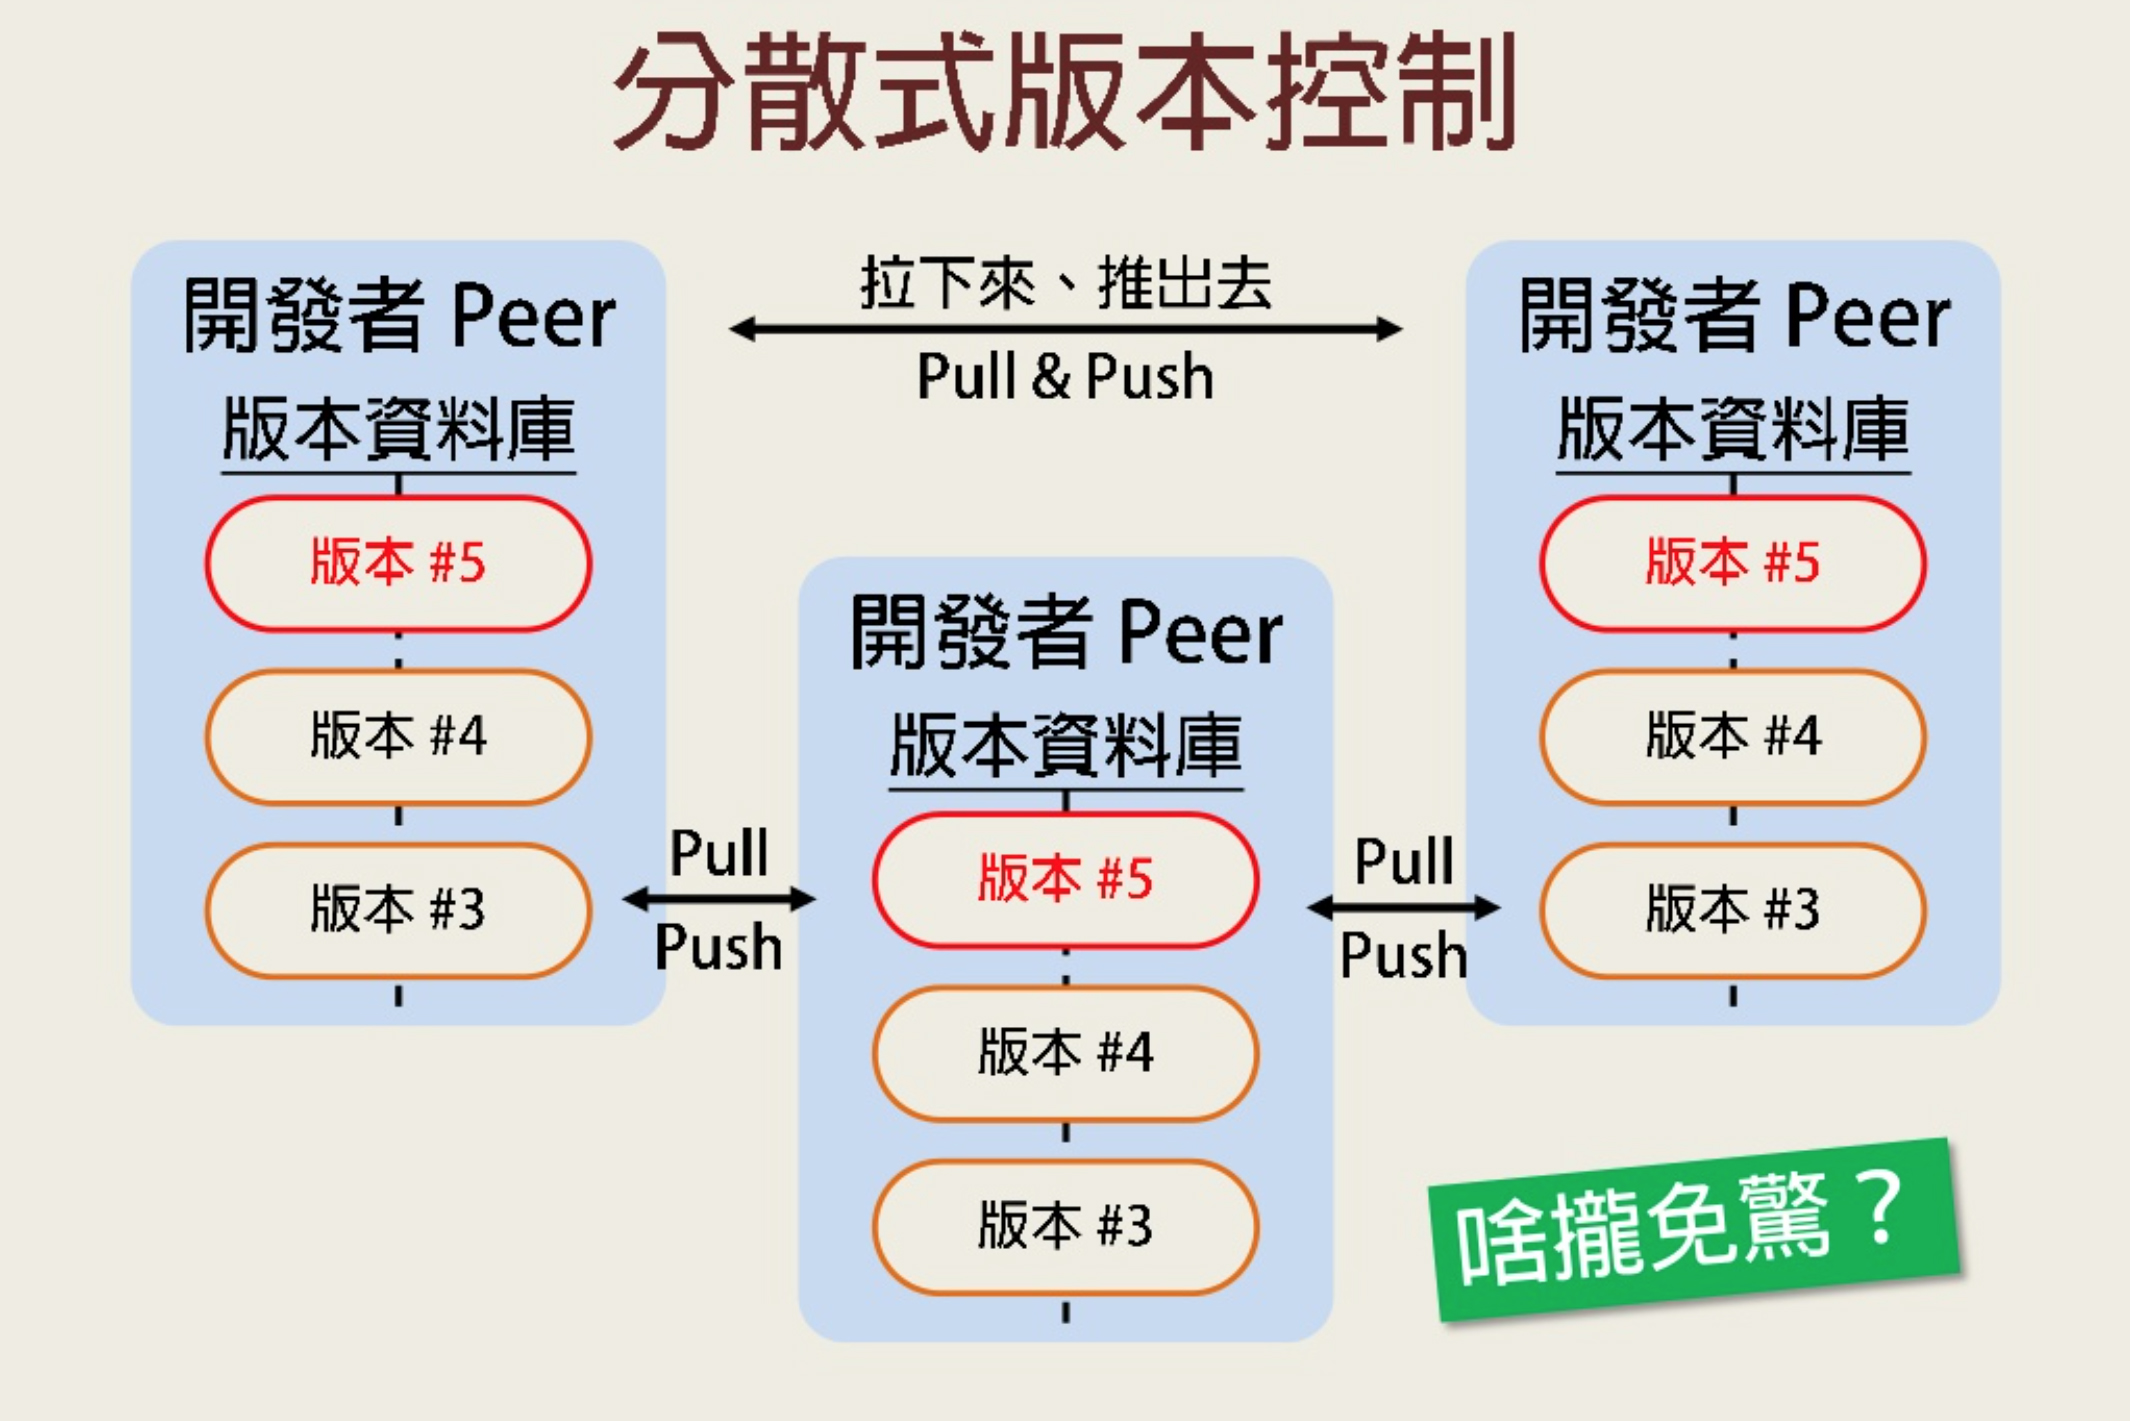
\includegraphics[width=0.8\textwidth]{images/003.jpg} 
          \caption{分散式版本控制}
        \end{figure}
      \end{frame}
    \end{subsection}
  \end{section}

  \begin{section}{Git}
    \begin{subsection}{簡介}
      %% normal frame
      \begin{frame}{Git}
        \begin{itemize}
          \item 發明人 Linus Torvalds (即Linux創始人)
          \item 目的為管理Linux程式碼
          \item 是一分散式版本控制
        \end{itemize}
      \end{frame}
      
      \begin{frame}{Git目標}
        \begin{itemize}
          \item 速度快
          \item 簡單使用
          \item 非線性開發
          \item 分散式開發
        \end{itemize}
      \end{frame}
    \end{subsection}
   \end{section}

\end{document}
